\documentclass[pdf,aspectratio=169]{beamer}
\usepackage[]{hyperref,graphicx,siunitx,lmodern,booktabs}
\usepackage{physics}
\usepackage{em-commands}
\mode<presentation>{\usetheme{EM}}

\graphicspath{ {../Images/} }

\sisetup{per-mode=symbol}

%preamble
\title{In fond rememberance\ldots}
\date{August 27, 2018}
\author{Jed Rembold}

\begin{document}
\renewcommand{\theenumi}{\Alph{enumi}}

\begin{frame}{Welcome to Electromagnetics!}
  \begin{itemize}
	  \item Things to do before \alert{next class}:
	  \begin{itemize}
		  \item Check out the class webpage: \url{http://www.willamette.edu/~jjrembold/classes/wu345/main/}
		  \item Read over syllabus
		  \item Make sure you have the book and \textbf{read sections 1.2 and 1.3}
		  \item Get added to the class in Gradescope
			  \begin{itemize}
			  	\item Invite emails should be going out
			  \end{itemize}
		  \item Get added to the class in Campuswire
			  \begin{itemize}
			  	\item Invite emails should be going out
			  \end{itemize}
		  \item Bring a phone or something that can connect to internet 
	  \end{itemize}
  \item Things to do this \alert{week}
	  \begin{itemize}
		  \item Homework 1 is posted and WILL be due midnight on Monday (despite the holiday!)
		  \item Have Anaconda installed on a laptop you can bring to class on Friday
			  \begin{itemize}
			  	\item Ensure you can create or open a Jupyter Notebook
			  \end{itemize}
	  \end{itemize}
  \end{itemize}
\end{frame}

\begin{frame}{My Vitals}
  \begin{itemize}
	\item Office: Collins 311 (it's shared)
	\item Office Hours: M,W,Th 2-5pm \emph{and open door} ($\approx$always)
	\item Goudy Hours: M--Th 1-2pm near the windows in Goudy Commons
	\item Email: jjrembold@willamette.edu
	\item Phone: 503-370-6860
  \end{itemize}
\end{frame}

\begin{frame}{Important Stuff}
	\begin{itemize}
		\item Homework - 45\%
			\begin{itemize}
				\item Assignments due weekly on Monday at midnight
			\end{itemize}
		\item Midterms - 15\% each
			\begin{itemize}
				\item Exam 1: Oct 12 over Ch 1-3
				\item Exam 2: Nov 9 over Ch 4-5
			\end{itemize}
		\item Final - 25\%
			\begin{itemize}
				\item Dec 14
				\item Comprehensive
				\item Weighted heavily towards Ch 6-7
			\end{itemize}
	\end{itemize}
\end{frame}

\begin{frame}{Important Websites}
	\begin{itemize}
		\item The class website
			\begin{itemize}
				\item Where homework, and lecture slides will be posted
				\item Where the updated schedule will have reading requirements!
			\end{itemize}
		\item Gradescope
			\begin{itemize}
				\item Where all homework will be submitted as pdfs
				\item Please format homework questions with a new page for each problem
			\end{itemize}
		\item Campuswire
			\begin{itemize}
				\item Class forum for asking questions, responding to others questions, and general communication
				\item Reputation system can earn you some small amount of extra credit
			\end{itemize}
	\end{itemize}
\end{frame}

\begin{frame}{Computation}
	\begin{itemize}
		\item We will be using Python and Jupyter notebooks to add computation and visualization elements to this course
		\item If you don't already have it, I'll be getting installation instructions posted on the website
		\item Any computational elements you use in your homework should be printed to pdf and turned in along with the rest of your homework to Gradescope
		\item If you get stuck or have questions, post to Campuswire so others can benefit!
	\end{itemize}
\end{frame}

\begin{frame}{Advice}
	\begin{itemize}
		\item Read the assigned material before class, and submit major questions to Campuswire
		\item Go to class and participate in the questions and discussions
		\item Start your homework early to ensure it is making sense
		\item Don't work alone!
		\item Ask questions! Either in class or over Campuswire or in person.
	\end{itemize}
\end{frame}

\begin{frame}{}
	Thinking about your education and this course, which of the following is the most important to you?
	\begin{enumerate}
		\item Acquiring information (facts, principles, concepts, procedures, etc)
		\item Learning how to use information and knowledge in new situations?
		\item Developing lifelong learning skills
	\end{enumerate}
\end{frame}

\begin{frame}{}
	Our time together here is unfortunately rather limited. Which of these three goals do you think you can do on your own (before or after class)?
	\begin{enumerate}
		\item Acquiring information (facts, principles, concepts, procedures, etc)
		\item Learning how to use information and knowledge in new situations?
		\item Developing lifelong learning skills
	\end{enumerate}
\end{frame}

\begin{frame}{}
	\begin{center}
		\tikz{\node[rounded corners, fill=Red, text=white, inner sep=4mm] at (0,0) {So what is Phys 345 really about?};}\\
		\pause
		\vspace{1cm}
		Electromagnetics is the \underline{foundational} \emph{field theory} course of physics!
	\end{center}
\end{frame}

\begin{frame}{}
	Take 5 minutes with a partner to map out all the electromagnetic concepts you \emph{already know} (there are a lot!), and how they are related to one another.
\end{frame}

\begin{frame}{}
	In a typical Cartesian coordinate system, say vector $\va{A}$ lies along the $+\yhat$ direction and vector $\va{B}$ lies along the $+\zhat$ direction. In what direction would $\va{A}\cross\va{B}$ point?
	\begin{enumerate}
		\item $-\yhat$
		\item $-\xhat$
		\item $+\xhat$
		\item $-\zhat$
		\item Impossible to say without more info
	\end{enumerate}
\end{frame}

\begin{frame}{}
	How is vector $\pos_3$ related to $\pos_1$ and $\pos_2$?
	\begin{center}
		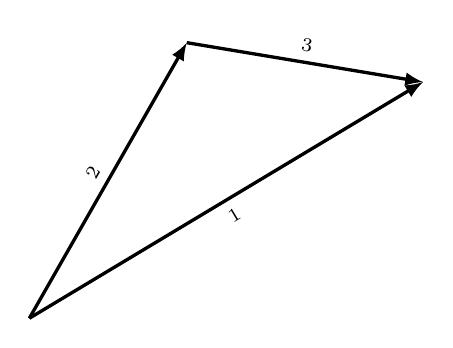
\begin{tikzpicture}
			\draw[very thick, -latex] (0,0) -- +(5,3) node[midway,below,sloped] {$\pos_1$};
			\draw[very thick, -latex] (0,0) -- +(2,3.5) node[midway,above,sloped] {$\pos_2$};
			\draw[very thick, -latex] (2,3.5) -- (5,3) node[midway,above,sloped] {$\pos_3$};
		\end{tikzpicture}
		\begin{enumerate}
			\item $\pos_3 = \pos_1 + \pos_2$
			\item $\pos_3 = \pos_1 - \pos_2$
			\item $\pos_3 = \pos_2 - \pos_1$
			\item None of these
		\end{enumerate}
	\end{center}
\end{frame}

\begin{frame}{}
	\begin{columns}
		\column{0.5\textwidth}
		In polar coordinates (so just 2D), what would be the correct description of the position vector $\pos$ of the point P shown at $(x,y) = (1,1)$?\\
		\begin{enumerate}
			\item $\pos = \sqrt{2} \vu{s}$
			\item $\pos = \sqrt{2} \vu{s} + \frac{\pi}{4}\vu*{\phi}$
			\item $\pos = \sqrt{2} \vu{s} - \frac{\pi}{4}\vu*{\phi}$
			\item $\pos = \frac{\pi}{4}\vu*{\phi}$
		\end{enumerate}
		
		\column{0.5\textwidth}
		\begin{center}
			\begin{tikzpicture}[scale=2]
				\draw[-latex] (-1,0) -- (2,0) node[below,math] {\xhat};
				\draw[-latex] (0,-1) -- (0,2) node[left,math] {\yhat};
				\node[point, label={below right:P}] (P) at (1,1) {};
				\node[point] (o) at (0,0) {};
				\draw[very thick, -latex] (o) -- (P) node[midway,below right, math] {\pos};
				\draw[very thick, -latex, Teal] (P) --+(45:.5) node[right,math] {\vu*{s}};
				\draw[very thick, -latex, Teal] (P) --+(45+90:.5) node[above,math] {\vu*{\phi}};
			\end{tikzpicture}
		\end{center}
		
	\end{columns}
\end{frame}






\end{document}
